\chapter{Progettazione e codifica}
\label{cap:progettazione-codifica}

\intro{In questa sezione vengono descritti tre processi fondamentali nello sviluppo software: la progettazione dell’interfaccia grafica, la realizzazione del PoC e la macro-fase di progettazione architetturale e codifica.}

\section{Mockup dell'interfaccia grafica}
\label{sec:mockup}

\par Durante la progettazione dell’interfaccia grafica, ho tratto ispirazione da diverse soluzioni esistenti analizzate nella fase preliminare. In particolare:
\begin{itemize}
    \item Lo stile delle informazioni in anteprima (come meta keywords, conteggio delle parole, ecc.) si ispira al layout dell’estensione \textit{Detailed SEO Extension}, al quale è stato aggiunto un comportamento flessibile per gestire dinamicamente lo spazio nella barra laterale;
    \item Il box di inserimento della parola chiave è il risultato di una combinazione tra le interfacce di \textit{MozBar} e \textit{Wincher}. Da \textit{MozBar} ho ripreso l’idea della checkbox posizionata sotto il campo di input, che permette di evidenziare una keyword senza dover eseguire preventivamente una ricerca o un’analisi. \textit{Wincher}, invece, ha ispirato il design del campo di testo affiancato da un pulsante per avviare l’analisi;
    \item L’organizzazione delle parole chiave in categorie (user-added keywords, meta keywords, most frequent keywords) si basa su un approccio integrato derivato da strumenti come \textit{Keyword Density Analyzer}, \textit{SEOquake}, \textit{SEOptimer} e \textit{SEO tester online}. Da questi strumenti ho ripreso anche l’idea di una rappresentazione dei risultati in formato tabellare;
    \item Il sistema di filtraggio delle parole chiave - non presente nella prima bozza dell’interfaccia - è stato ispirato da \textit{SEOquake}, che offre funzionalità simili per agevolare la consultazione dei risultati.
\end{itemize}

\vspace{10pt}
\par\noindent Le scelte progettuali sopra elencate sono state accompagnate da un’analisi dello spazio disponibile e delle \textit{best practice} in materia di design, con l’obiettivo di definire fin dalle prime fasi quali elementi utilizzare e come disporli sull’interfaccia per garantire comfort visivo ed evitare il sovraccarico cognitivo. Per la scelta cromatica, il punto di partenza è stato il colore più distintivo, il viola, attorno al quale è stata costruita una combinazione di colori coerente e conforme alle linee guida \gls{wcag}. Questi concetti sono stati infine tradotti in un mockup realizzato con \textit{Figma}.

\begin{figure}[H]
    \centering 
    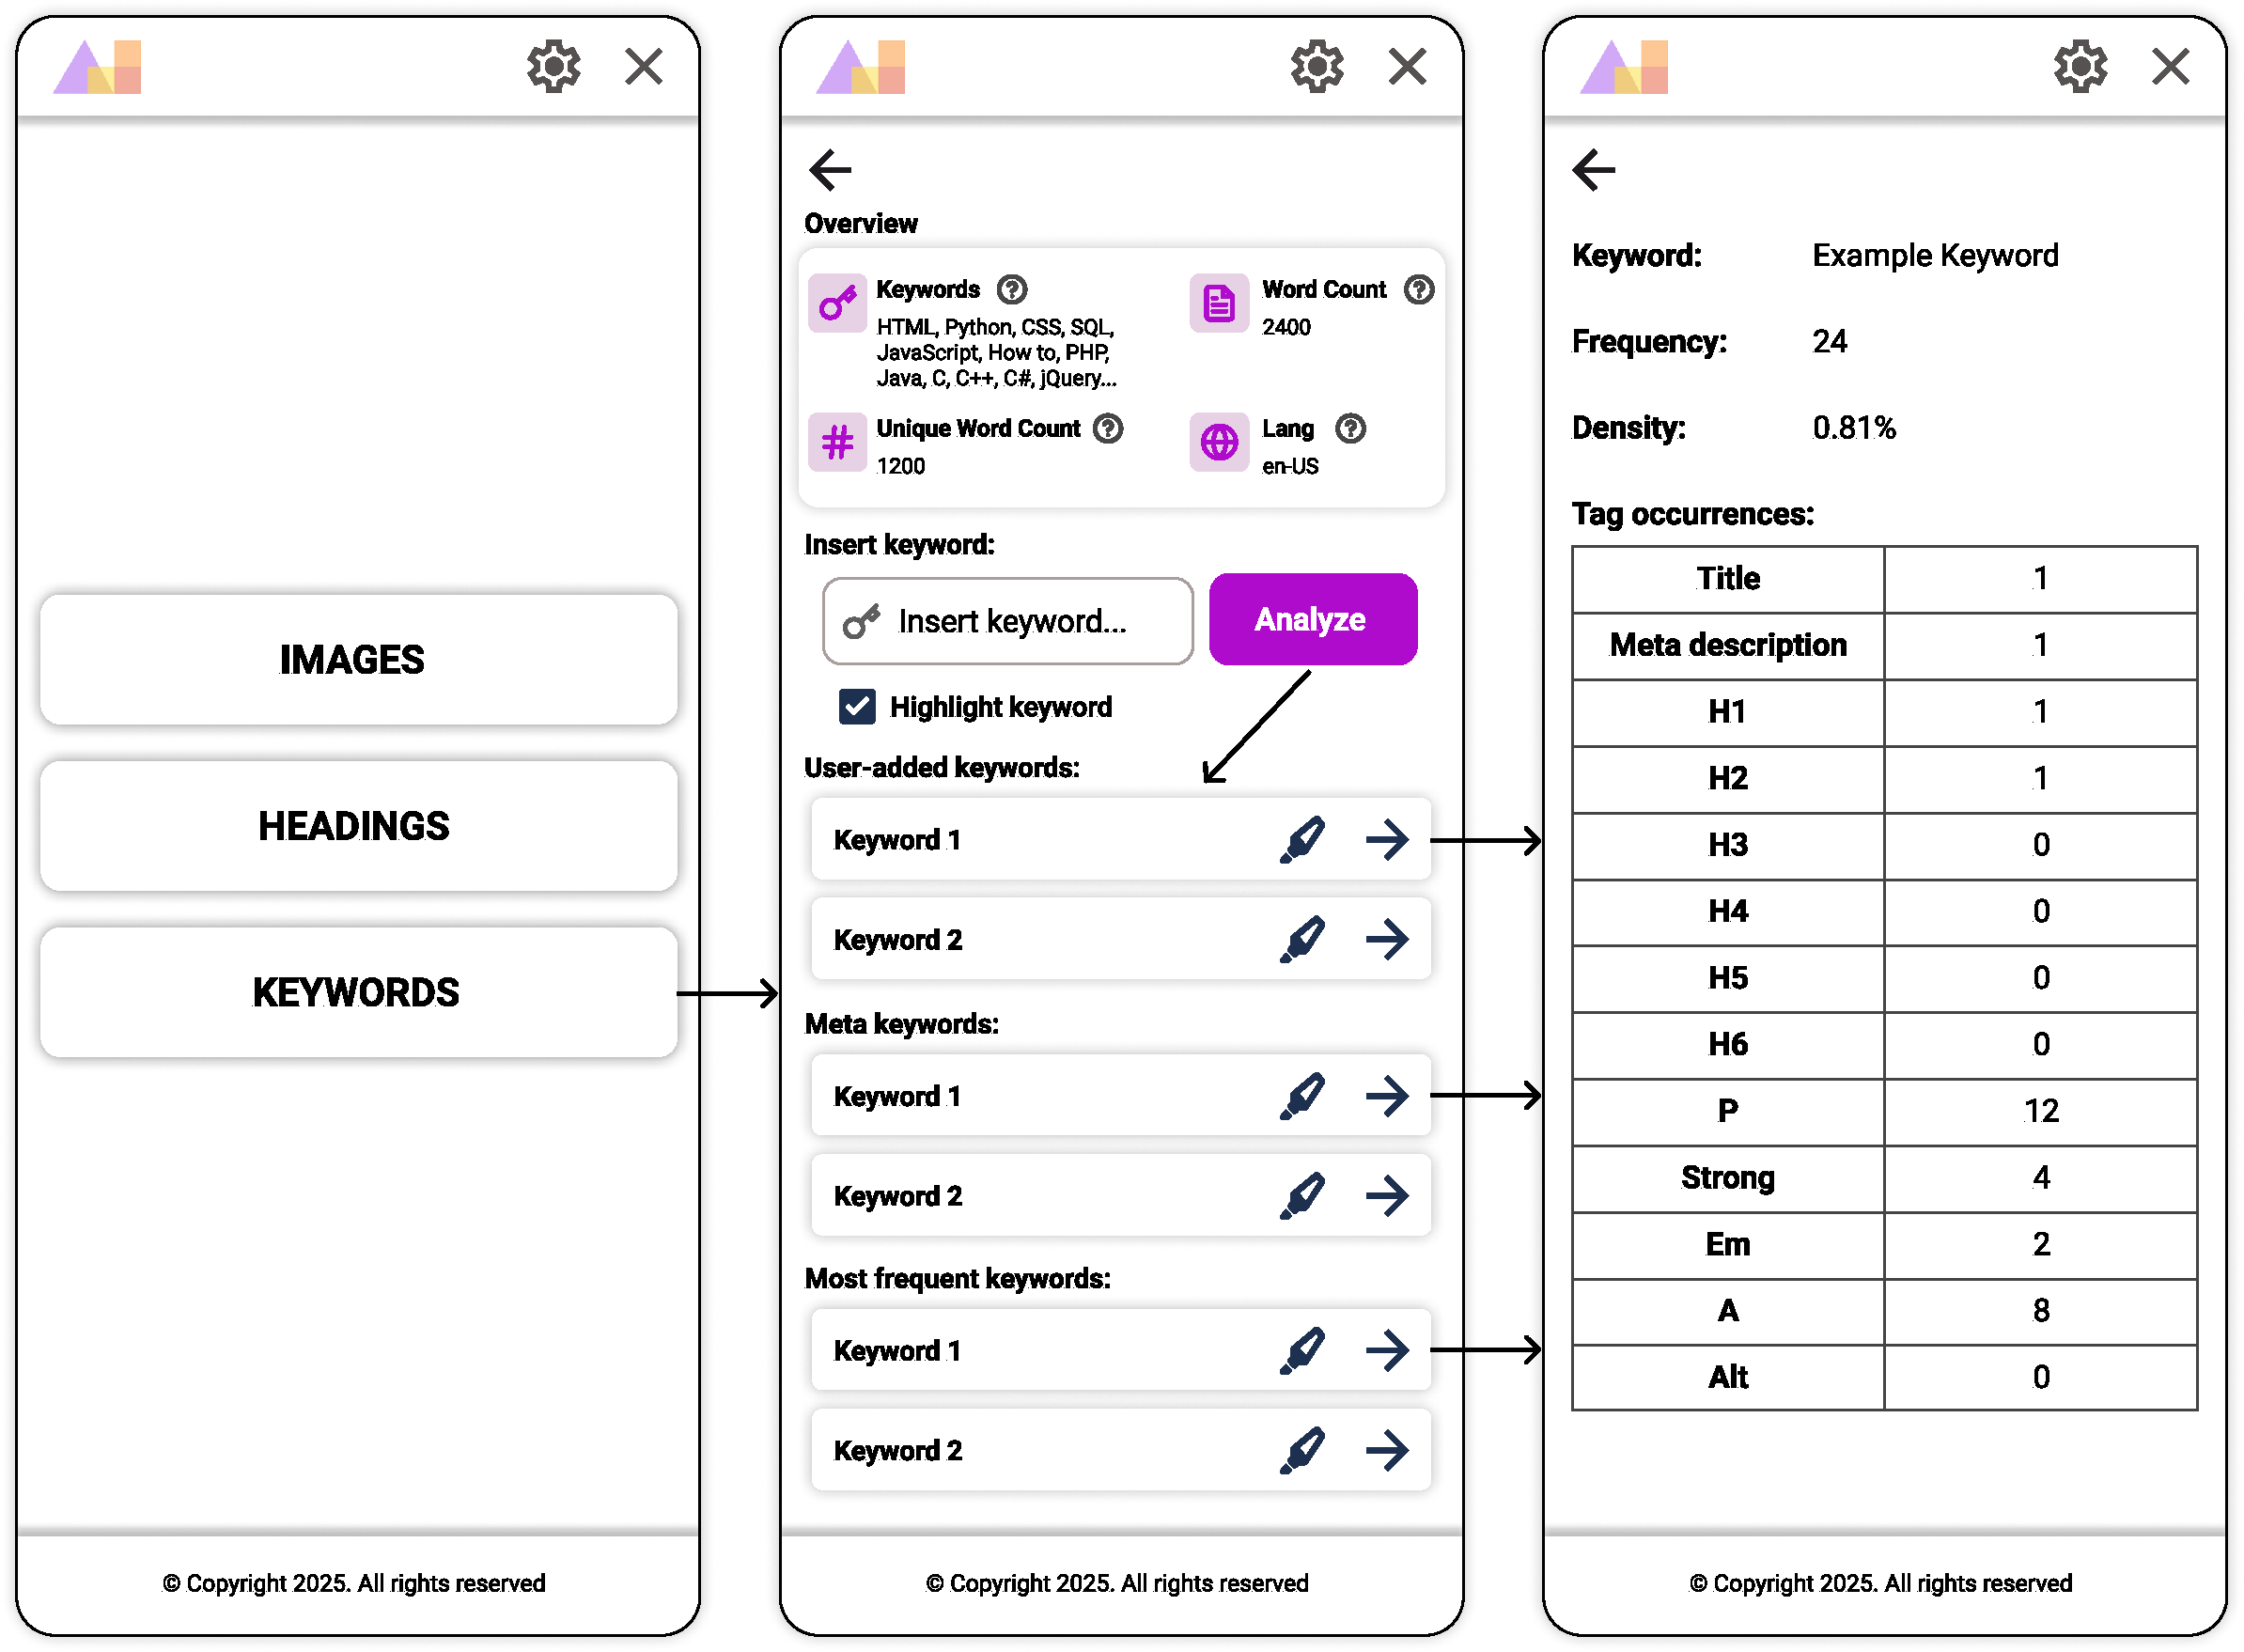
\includegraphics[width=\columnwidth]{progettazione/mockup.pdf} 
    \caption{Mockup dell'interfaccia grafica}
\end{figure}

\section{PoC}
\label{sec:poc}

\par Lo scopo principale del \gls{poc} è stato quello di tradurre in codice il mockup dell’interfaccia grafica, al fine di verificare la correttezza e la coerenza delle scelte progettuali. Per raggiungere questo obiettivo, ho simulato il funzionamento dell’estensione in ambiente \gls{localhost}, sostituendo una pagina reale con una versione statica. Questa soluzione ha reso possibile lavorare in un ambiente di test controllato, all’interno del quale è stato possibile condurre uno studio di fattibilità e sperimentare le funzionalità di analisi ed evidenziazione visiva delle parole chiave. Al termine di questa fase, è stato organizzato un incontro con la Proponente per discutere i risultati ottenuti e le problematiche riscontrate, e identificare gli elementi da mantenere, modificare o integrare, in vista della successiva progettazione architetturale e dello sviluppo definitivo.

\section{Progettazione architetturale}
\label{sec:progettazione}

\begin{figure}[H] 
    \centering 
    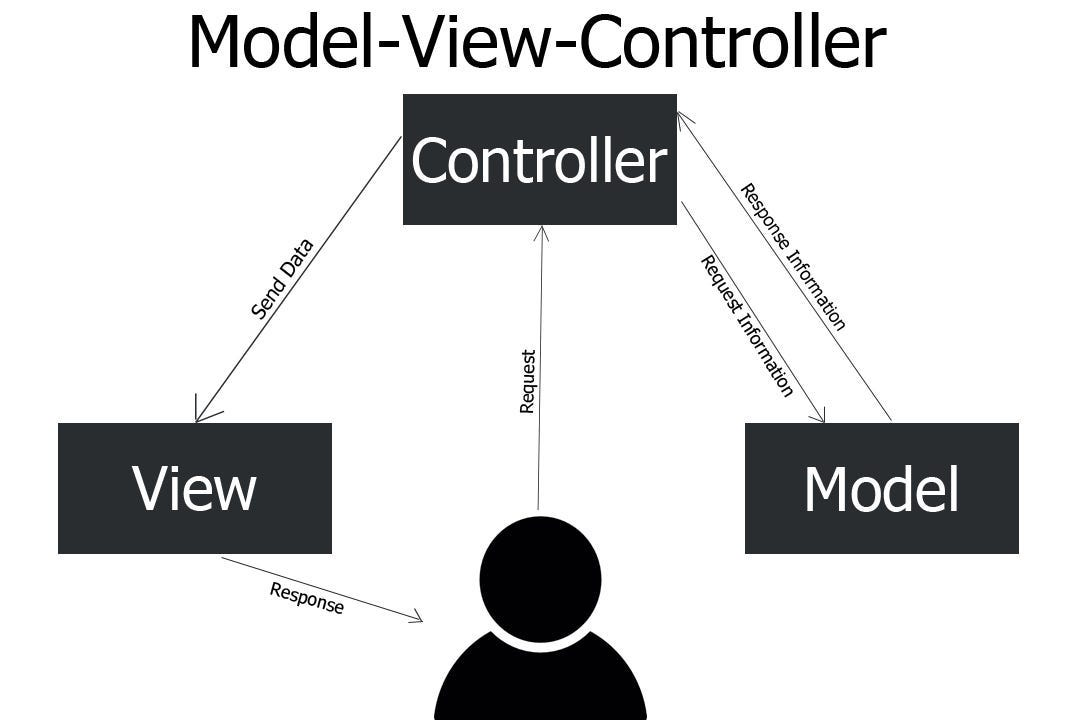
\includegraphics[width=0.8\textwidth]{progettazione/mvc.jpg} 
    \caption{Pattern MVC (Model-view-controller)}
\end{figure}

\par\noindent Di seguito è riportata la struttura della funzionalità di analisi delle parole chiave:

\vspace{10pt}
\begin{samepage}
  \dirtree{%
    .1 .github.
    .2 workflows.
    .1 keyword.
    .2 controller.
    .2 model.
    .2 services.
    .3 strategy.
    .2 tests.
    .2 utils.
    .2 view.
    .1 static.
    .2 fonts.
    .2 img.
    .2 libs.
  }
\end{samepage}

\section{Design Pattern utilizzati}
\label{sec:design-pattern}

\section{Elenco delle classi}
\label{sec:elenco-classi}
